\documentclass[12pt]{article}
\title{Elektrotechnik 2 \\ Notizen }
\author{K L U K}
\usepackage{amsmath}
\usepackage{graphicx}
\usepackage[utf8]{inputenc}
%\usepackage{MnSymbol}
\begin{document}
\maketitle 
\newpage
\section{19. Globale und lokale Eigenschaften magnetischer Felder}
\subsection{Der Satz vom magnetischen Hüllenfluss}
Globale Eigenschaft magn. Flussverteilung:
\begin{equation}\label{key}
\phi(\partial \mathcal{V}) = 0
\end{equation}
Darstellung magn. Flüsse als Flächensumme der Flussdichte: 
\begin{equation}\label{key}
\phi(\mathcal{A}) = \int_{\mathcal{A}} B_n dA
\end{equation}
als Kurvensumme des Vektorpotentials: 
\begin{equation}\label{key}
\phi(\mathcal{A})=\int_{\partial \mathcal{A}} A_s ds
\end{equation}
Kommentar von Peter: 
\begin{equation}\label{key}
d\vec{s} = \vec{e_s} ds  \quad \vec{e_s}\cdot \vec{A} = |\vec{A}|\, cos(\alpha) = A_s 
\end{equation}
\paragraph{Verhalten der magnetischen Flussdichte an einer Sprungfläche}

\begin{equation}\label{key}
G^+-G^-=\lsem G \rsem
\end{equation}
\paragraph{Verhalten des magnetischen Vektorpotentials an einer Sprungfläche} %19:21
An einer Sprungfläche ist die \textbf{Tangentialkomponente } des magnetischen Vektorpotential \textit{stetig}. 

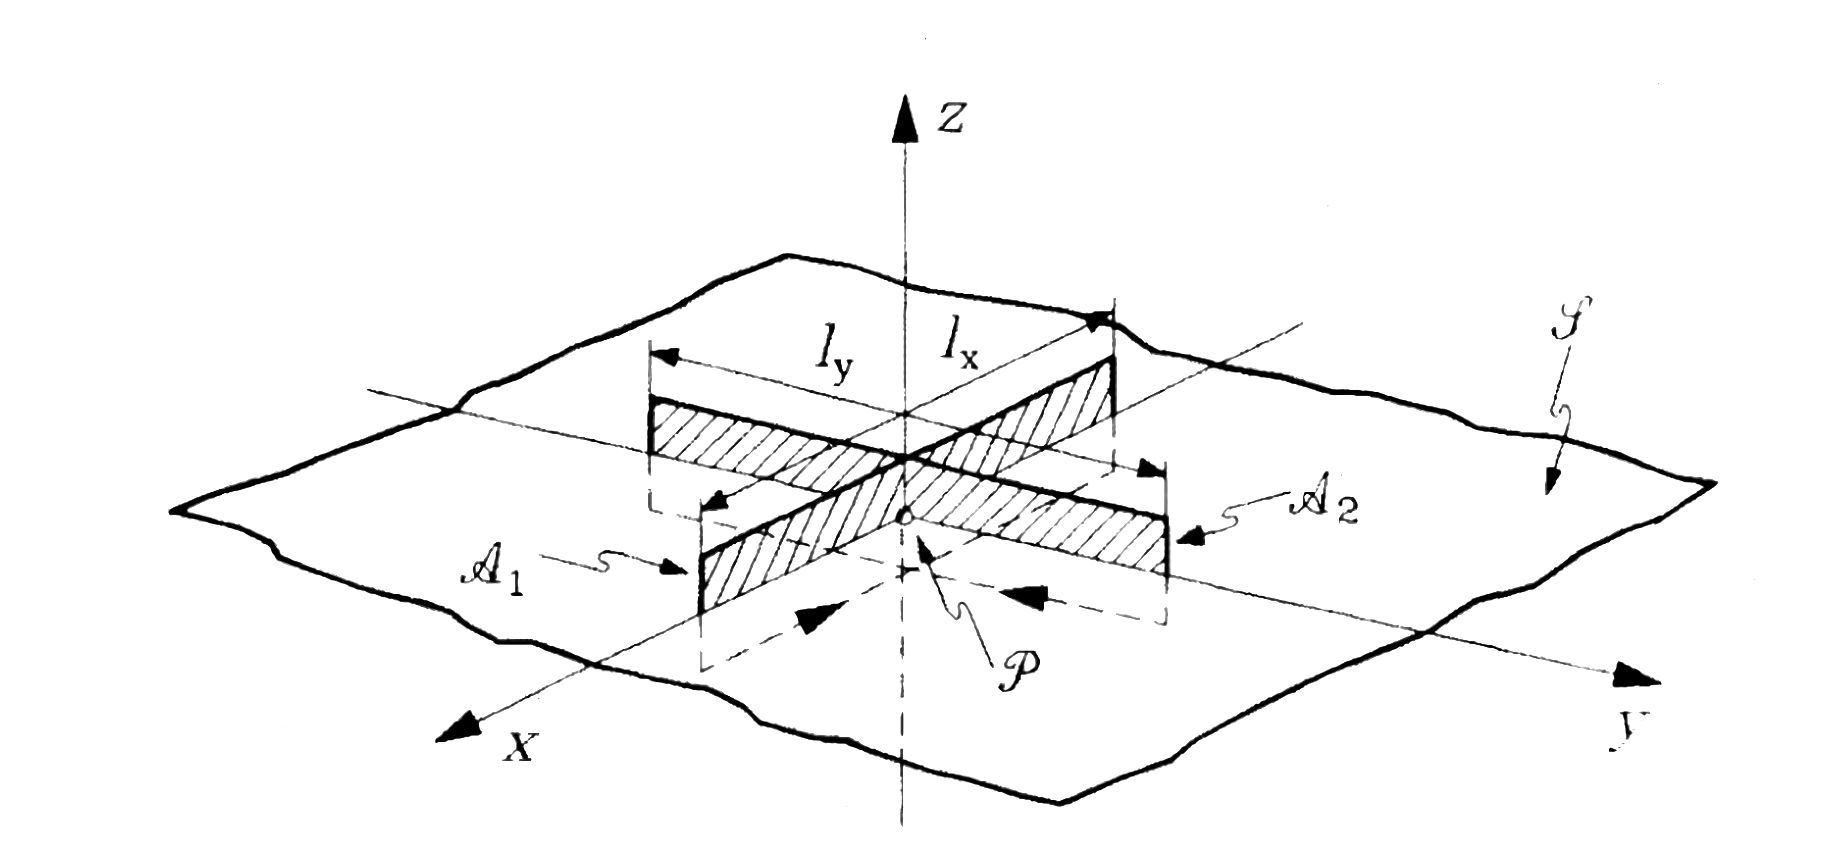
\includegraphics[width=15cm]{pic/abb14-5x2nr}
\begin{equation}\label{key}
\vec{A} = \vec{A}_n + \vec{A}_t
\end{equation}
\begin{equation}\label{key}
\vec{A}_n = A_z \vec{e}_z
\end{equation}
\begin{equation}\label{key}
\vec{A}_t = A_x \vec{e}_x + A_y \vec{e}_y
\end{equation}
\begin{equation}\label{key}


\lsem \vec{A_t} \rsem = \vec{0}

\end{equation}
Kommentar Peter: 
\begin{equation}\label{key}
\vec{A}_t = A_x \vec{e}_x + A_y \vec{e}_y
\end{equation}
\subsection{Der Durchflutungssatz}

Globale Eigenschaft stationärer Stromverteilungen Näherungsweise Gültig für quasi-stationäre Stromverteilungen. 

\begin{equation}\label{key}
V(\partial \mathcal{A})= I (\mathcal{A}) = \Theta(\mathcal{A})
\end{equation}
\noindent
Darstellung magnetischer Spannungen als Kurvensumme der Feldstärke:
\begin{equation}\label{key}
V(\mathcal{C}) = \int_{\mathcal{C}} H_s ds
\end{equation}
\noindent
Darstellung elektrischer Ströme als Summe von Linienströmen: 
\begin{equation}\label{key}
I(\mathcal{A}) = \sum_k I_k 
\end{equation} %es gibt noch K und J 
Kommentar Peter: \\ 
\noindent
Spezielles \(\mathcal{C}\) daraus folgt:  \begin{align}
\mathcal{C}&=\partial \mathcal{A}\\
\partial \mathcal{C} &= \partial  \partial \mathcal{C} = 0
\end{align}
\(H_s\) leitet sich aus: 
\begin{equation}\label{key}
\vec{e}_s \cdot \vec{H}_s = | \vec{H}| \cdot cos(\alpha) = H_s 
\end{equation}
\paragraph{Verhalten der magnetischen Feldstärke an einer Sprungfläche} %35:17
\begin{figure}
\centering
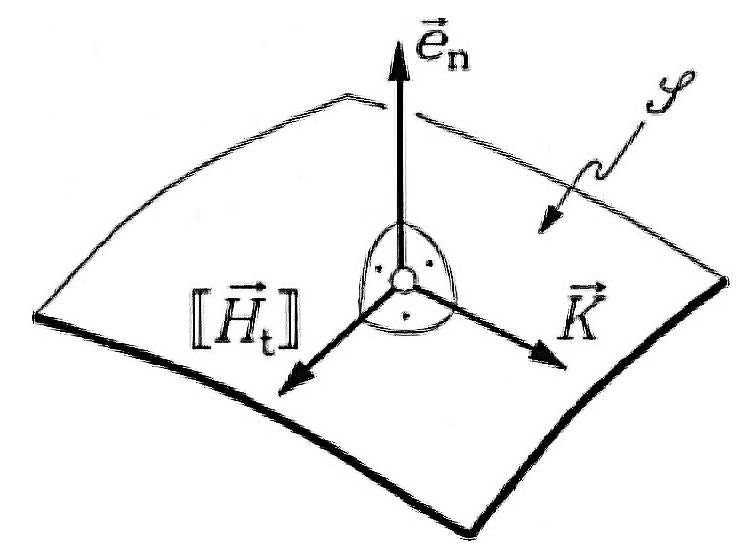
\includegraphics[width=5cm]{pic/abb19-3x2nr}
\end{figure}

\begin{align}
\vec{H} &= \vec{H}_n + \vec{H}_t\\
\vec{H}_n &= H_z \vec{e}_z \\
\vec{H}_t &= H_x \vec{e}_x + H_y \vec{e}_y \\
\vec{K} &= K_x \vec{e}_x + K_y \vec{e}_y \\
\vec{e}_n \times \lsem \vec{H} \rsem = \vec{K}
\end{align}
\newpage
\subsection{Materialgleichungen}
Die Oberfläche eines ideal magnetisierbaren Körpers: 
\begin{align}
\vec{H}^- = \vec{0},\; \vec{H}^+=\vec{K}\times \vec{e}_n
\end{align}
Woebi für \(\vec{K} = \vec{0}\) gilt speziell: \(\vec{H}^+ = \vec{0}\), dabei steht \(\vec{H}^+\) senkrecht an der Oberfläche. \\
\noindent \\
Grenzflächen zwischen zwei magnetisch isotropen Körpern mit \(\vec{B}^\pm = \mu^\pm \vec{H}^\pm\) 

\begin{align}
\vec{B}_n^+ = \vec{B}^- \\
\vec{B}^+_t = \frac{\mu^+}{\mu^-}\left( \vec{B}^-_t + \mu^- \vec{K} \times \vec{e}_n \right)\\
\vec{H}_n^+ = \frac{\mu^-}{\mu^+}\vec{H}_n^-\\
\vec{H}_t^+ = \vec{H}_t^- + \vec{K} \times \vec{e}_n
\end{align}
\newpage 

% % % % % % % % % % % % % % % % % % % %






% % % % % % % % % % % % % % % % % % % %
\section*{28. Energie im Elektromagnetismus}
\subsection{Energiespeicherung }
Der ideale Kondensator speichert die Energie mit folgender Beziehung: 
\begin{equation}\label{key}
I = C\dot{U},\quad P(t) = U(t) I(t) = C U(t) \dot{U}(t)
\end{equation}
\noindent
Der Energieerhalt wird beschrieben durch: 
\begin{equation}\label{key}
W_c = \frac{CU^2}{2}=\frac{QU}{2}=\frac{Q^2}{2C}
\end{equation}

\paragraph{Eigenschwingungen}
Eigenschwingung bedeutet ein ständiger Energieaustausch zwischen unabhängigen Energiespeichern. 

\begin{align}
\dot{U}=-I/C, \quad  U(0) = \hat{U} \\
\dot{I}=U/L, \quad I(0) = 0 
\end{align}
\end{document}